%%%%%%%%%%%%%%%%%
\section{Classificação Associativa}\label{sec:ca}
%%%%%%%%%%%%%%%%%

A classificação associativa (CA) integra conceitos de mineração de regras de associação e classificação supervisionada, utilizando regras para representar o conhecimento extraído dos dados. Diferentemente da mineração tradicional de regras de associação, que busca identificar relações entre itens sem necessariamente considerar uma variável-alvo, a CA utiliza regras de associação de classe (RACs), cujo consequente corresponde a uma classe do problema \cite{liu1998}. Uma RAC é representada por $A \Rightarrow c$, em que $A$ é um conjunto de condições sobre os atributos e $c$ é um rótulo de classe.

Para compreender a construção dessas regras, considera-se um conjunto de dados $D$ formado por $N$ instâncias e um conjunto de itens $I=\{i_1,\ldots,i_m\}$. Em dados tabulares, um item representa, em geral, uma condição do tipo <atributo=valor>, como <cor=azul>. Um conjunto de itens (\textit{itemset}) corresponde a uma combinação dessas condições. Cada instância pode ser representada pelos itens associados aos valores de seus atributos e por sua classe. Na regra $A \Rightarrow c$, o antecedente $A \subseteq I$ corresponde a um \textit{itemset}, enquanto o consequente $c$ identifica a classe prevista.

As regras são usualmente avaliadas por medidas objetivas, entre as quais se destacam o suporte e a confiança \cite{apriori}. Para uma RAC $A \Rightarrow c$, o suporte expressa a proporção de instâncias em que as condições de $A$ ocorrem juntamente com a classe $c$, enquanto a confiança representa a proporção de instâncias que satisfazem $A$ e pertencem à classe $c$. Essas medidas são definidas, respectivamente, pelas Equações~\ref{eq:suporte} e~\ref{eq:confiança}, em que $n(A,c)$ indica o número de instâncias que satisfazem $A$ e pertencem à classe $c$, e $n(A)$ indica o número de instâncias que satisfazem $A$.

\begin{equation}
\text{Suporte}(A \Rightarrow c) = \frac{n(A,c)}{N} = P(A,c)
\label{eq:suporte}
\end{equation}

\begin{equation}
\text{Confiança}(A \Rightarrow c) = \frac{n(A,c)}{n(A)} = P(c\mid A)
\label{eq:confiança}
\end{equation}

Na extração de regras, valores mínimos de suporte (\textbf{sup-min}) e confiança (\textbf{conf-min}) podem ser estabelecidos para restringir os padrões considerados. Em algoritmos baseados no Apriori \cite{apriori}, a busca explora combinações de itens, identificando conjuntos frequentes e gerando regras que atendem aos critérios definidos \cite{agrawal1993mining,apriori}. O número de combinações possíveis cresce com a quantidade de itens disponíveis, podendo alcançar $2^{|I|}$ subconjuntos, incluindo o conjunto vazio, antes da aplicação de restrições e estratégias de poda. Assim, o aumento da dimensionalidade e a presença de atributos com muitos valores podem ampliar o espaço de busca. Essa característica ajuda a explicar a relevância da seleção de atributos como etapa anterior à indução de classificadores associativos.

Os algoritmos de CA diferem quanto às estratégias de geração, ordenação (ranqueamento) e poda das regras \cite{10.1016/j.eswa.2025.127454}. A representação baseada em RACs permite que os padrões empregados pelo classificador sejam inspecionados por especialistas, embora a quantidade e a extensão das regras também influenciem a complexidade do modelo. A literatura apresenta diferentes algoritmos e implementações de CA, incluindo o CBA, proposto por \citeonline{liu1998}, e pacotes que disponibilizam classificadores associativos para uso geral \cite{Hahsler2019254,Padillo2020,10.1145/3419604.3419762}. Uma visão recente dessa família de métodos é apresentada em \citeonline{10.1016/j.eswa.2025.127454}.

No CBA, a construção do classificador compreende, de maneira geral, três etapas: (a) extração de RACs; (b) ordenação (ranqueamento) das regras; e (c) poda das regras para composição do modelo. Na primeira etapa, o algoritmo emprega uma adaptação do Apriori para obter regras de associação de classe que satisfaçam os critérios de suporte e confiança estabelecidos \cite{liu1998}. As etapas seguintes podem ser sintetizadas da seguinte maneira:

\begin{description}
    \item[Ranqueamento.] As RACs extraídas são ordenadas por uma relação de precedência $\succ$. Dadas duas regras $r_i$ e $r_j$, considera-se $r_i \succ r_j$ quando: (i) a confiança de $r_i$ é maior que a de $r_j$; (ii) em caso de empate na confiança, o suporte de $r_i$ é maior; ou (iii) em caso de empate em ambas as medidas, $r_i$ foi gerada antes de $r_j$.

    \item[Poda.] A partir da lista ordenada, o CBA utiliza a cobertura das instâncias de treinamento e os erros de classificação para selecionar as regras que compõem o classificador final, juntamente com a classe \textit{default}.
\end{description}

Na predição, dada uma instância não vista, o classificador percorre as regras ordenadas e atribui a classe associada à primeira regra cujo antecedente é satisfeito pela instância. Caso nenhuma regra seja aplicável, utiliza-se a classe \textit{default} definida durante a construção do classificador. A Figura~\ref{fig:fluxo_cba} ilustra o fluxo geral de indução e predição.

\begin{figure}[H]
    \centering
    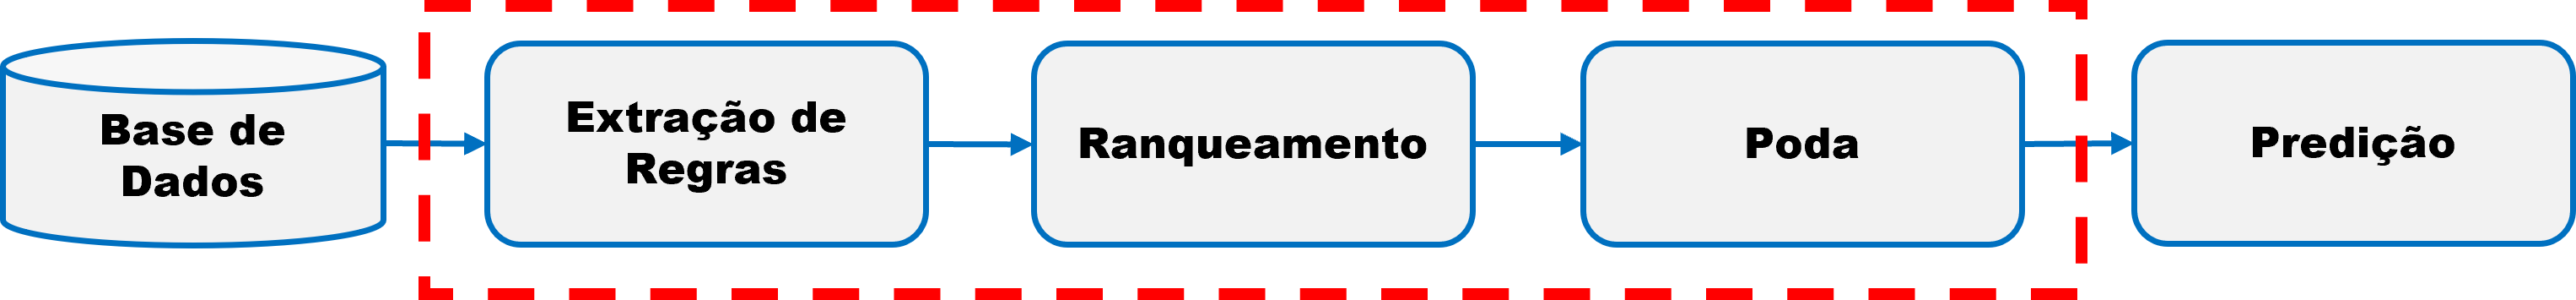
\includegraphics[width=\linewidth]{figuras/fluxo-geral.png}
    \caption{Fluxo geral de indução e predição de um classificador associativo.}
    \label{fig:fluxo_cba}
\end{figure}

No contexto desta dissertação, a seleção de atributos é realizada antes da indução do classificador associativo. Dessa forma, a redução do conjunto de atributos pode alterar os itens disponíveis para a geração de RACs e, consequentemente, influenciar tanto o desempenho preditivo quanto a quantidade e a estrutura das regras produzidas. Esses efeitos motivam a avaliação conjunta do desempenho e da complexidade dos classificadores obtidos após a aplicação do EFS4AC.
